

\chapter{Experimental Setups}\label{appendix:setups}
The systems that were used in the conducted experiments are described in the following, focusing on the media processing and required details to reproduce the technical conditions.
It must be noted that the systems for experiments \E1{}, \EIIa{}, \EIIb{}, and \E3{} were designed especially for use in a laboratory setting and thus focused on a precise presentation of the performance levels.
The systems implemented for experiments \E4{}, \E5{}, and \E6{} were designed for use in field experiments, and thus ease of setup, reliability, and robustness was required.

\section{Experiment E1}
For \E1{}, two systems were required.
First, a listening-only training was conducted, presenting typical speech telephony degradations.
For the multi\-/episodic assessment, a two-party speech telephony system was required.

\subsection{Listening-only Training}
The listening-only training was conducted with a tablet computer (\emph{Fujitsu~Stylistic~ST6012}).
For diotic representation, a pair of \emph{AKG~K\=/271} headphones was connected to the internal sound card of the tablet computer.
The system was calibrated using a \emph{HEAD acoustics} head and torso simulator \emph{HSM~II.3} (sound pressure level of \unit[75]{dB20$\mu$Pa}; babble noise).
The stimuli were generated with the \textsc{\lowercase{ITU\=/T}~\lowercase{STL2009}} tools \citep{itu-t_recommendation_g.191_software_2010} and the audio-processing tool \textsc{\lowercase{SOX}}\footnote{The \textsc{\lowercase{SOX}} project is hosted under \url{http://sox.sourceforge.net}.}.
The \textsc{\lowercase{STL2009}} were used for coding \textsc{\lowercase{G.711}} and \textsc{\lowercase{G.722}}~(Mode~1), and inserting packet loss for \textsc{\lowercase{G.722}}~(Mode~1, \acs{PLC} Mode~0).
\textsc{\lowercase{SOX}} was used for coding \textsc{\lowercase{GSM\=/FR}} and \textsc{\lowercase{LPC\=/10}} as well as for filtering wideband, narrowband, and white noise.

\subsection{Two-party Speech Telephony}
For the multi\-/episodic assessment of \E1{}, a speech telephony system for two-party conversations was required.

\paragraph*{Network-based Setup}
In the first part of \E1{}, a \ac{VoIP}\=/based system consisting of three computers was used.
These three computers were connected via Ethernet (\textsc{\lowercase{CAT\=/5}}). 
One computer (\emph{Lenovo~X61}) acted as a Server running the open-source telephony software \emph{Asterisk~11}\footnote{The Asterisk project is hosted under \url{http://www.asterisk.org}.}.
Two \emph{Fujitsu~Lifebook~S761} were running each a customized client based on \emph{PJSIP~2.1}\footnote{PJSIP is an open-source library for \acs{SIP}\=/based \ac{VoIP} (\url{http://www.pjsip.org}).}, which connected via \ac{SIP} to the server.
The clients presented only a minimal user interface, consisting of one button for call initiation and hangup, one button to set the current presence status, and a presence status indicator for the remote client.
Call initiation was only possible if both clients set their presence status to available.
The two clients could not communicate directly with each other as the Asterisk server acted as a proxy.
Transmission of the speech signal between Asterisk and the clients (both directions) was lossless by using the \emph{\textsc{\lowercase{L16}}} codec (sampling rate: \unit[16]{kHz}).
Asterisk applied the desired performance level, \ie, the selected codec, by compressing the signal and immediately decompressing it before relaying the signal.\footnote{The performance levels were set by using the transcoding capability of Asterisk. On an incoming call coded with \textsc{\lowercase{L16}}, Asterisk initiated a call to himself with the desired codec (\ie, \textsc{\lowercase{G.722}}, or \textsc{\lowercase{LPC\=/10}}). This second call triggered then an outgoing call to the callee encoded in L16.}
This system achieved a one-way end-to-end delay of \unit[120]{ms}.

On each of the two client computers, one \emph{Beyerdynamic~DT~790~Pro} headset connected to one \emph{Edirol~UA\=/25EX} sound card was used for recording and diotic reproduction.
Before starting the experiment, the output on both clients was once calibrated to a comfortable listening level by the experimental supervisor.

\paragraph*{Sound card Setup}
The network-based setup was replaced later by a more elaborate system, which provided easier setup and reduced the complexity for verification.
For this system, only one computer without an actual network was used.
Rather than transmitting the signals via Ethernet, an analogue transmission via audio cables was used.
Here, also the \emph{Beyerdynamic~DT~790~Pro} headsets were used.
The two headsets were connected to the processing computer (\emph{Lenovo~X61}) with one \emph{Edirol~UA\=/25EX} sound card.
The signal of each microphone was amplified with a \emph{RME~QuadMic~II} microphone preamplifier to counter potential signal loss due to the cable length of \unit[10]{m}.

On the processing computer \emph{PureData}\footnote{The PureData project is hosted under \url{https://puredata.info/}.}, an open-source audio processing application, was used to modify the speech signals.
As no speech codecs were available in PureData, the application was extended with the speech codecs \textsc{\lowercase{G.711}}, \textsc{\lowercase{G.722}}~(Mode~1), and \textsc{\lowercase{LPC\=/10}}.
It was verified that the PureData setup provides similar characteristics as the network-based setup.
The overall system achieved a constant, glitch-free one-way end-to-end delay of \unit[70]{ms}.
Before starting the experiment, the output was once calibrated to a comfortable listening level by the experimental supervisor.

\paragraph*{Additional Processing}
Due to the performance of the \emph{Beyerdynamic~DT~790~Pro} headsets, which provide a pair of closed headphones as well as a directional microphone, neither echo cancellation nor denoising algorithms were applied.
Both systems were configured to provide neither side tone nor comfort noise if not introduced by the codec.
No additional audio processing was applied.
The participants were located in two sound-insulated test rooms which met the requirements according to \citet{itu-t_recommendation_p.800_methods_1996}.

\section{Experiments E2a, E2b, and E3}
For the experiments \EIIa{}, \EIIb{}, and \E3{}, audio signals were presented with a pair of \emph{Sennheiser~HD~25\=/1} headphones.
For \EIIa{} and \E3{}, these were connected to the internal sound card of a \emph{Microsoft~Surface~Pro} tablet computer.
For \EIIb{}, these were connected to the internal sound card of a \emph{Nexus~7~(2013)}.
In all three experiments, the sound pressure level was calibrated to \unit[75]{dB20$\mu$Pa} using a \emph{HEAD acoustics} head and torso simulator \emph{HSM~II.3}.
The experiments were conducted in a sound-proof cabin following \citet{itu-t_recommendation_p.800_methods_1996}.
In \EIIb{}, the \ac{VoD} service was presented on the display of the Nexus~7, presenting the videos horizontally in full screen.
The brightness of this \unit[7]{inch} display was set to maximum without applying any device-specific color adaptation.

For these three experiments, non-degraded recordings of the two-party conversations conducted in \E1{} were selected.
These recordings were processed with the \textsc{\lowercase{ITU\=/T}~\lowercase{STL2009}} tools \citep{itu-t_recommendation_g.191_software_2010} for coding \textsc{\lowercase{G.722}} and with \textsc{\lowercase{SOX}} for coding \textsc{\lowercase{LPC\=/10}}.
For \EIIb{}, the video material was cut with \emph{Adobe~Premiere~6} and exported with H.264 (\unit[1280$x$720]{px}, \unit[5]{Mbit/s}, two-pass) and \acs{AAC} (\unit[448]{kbit/s}, stereo).
Subsequently, the video material was processed with \emph{FFmpeg}\footnote{The FFmpeg project is available at \url{https://www.ffmpeg.org/}.} to apply the desired \acs{QP} factor while leaving the audio unchanged.

\section{Experiment E4}
\E4{} was the first experiment for this thesis conducted as a field experiment with a usage period of multiple days.
For \E4{}, a speech telephony service and a \ac{VoD} service were implemented, which could be used by participants with their own personal computer and Internet access.
For recording and audio reproduction, each participant was equipped with a \emph{Logitech~P120} headset.

\subsection{Speech Telephony Service}
For conducting \E4{}, a publicly reachable \ac{VoIP} telephony service was set up.
The service needed to allow multiple two-party speech conversations at the same time while being able to insert packet loss for individual conversations.
For this service, one server was installed in the data center of \emph{Technische Universität Berlin}.
As operating system \emph{FreeBSD~9.0} was selected, because it provides a built-in firewall with a traffic shaper, \ie, \emph{Dummynet}~\citep{rizzo_dummynet:_1997}.
This traffic shaper allows to add network impairments (packet loss, delay, and jitter) per individual connection, \ie, protocol, port, and address.
On this server, the \ac{VoIP} software \emph{Asterisk~10} was installed, which was configured to act as a \ac{SIP} registrar as well as \acs{RTP}\=/relay for the \acs{UDP}\=/based media streams.
On call initiation of a client, Asterisk informed Dummynet about the desired packet loss rate for the media streams of this call.
Packet loss was not inserted to the \ac{SIP} connections between clients and server, because this affects the reactivity of the telephony system and might lead to call drops.
On each participant's computer, the \ac{VoIP} client \emph{Jitsi~1.0} was installed.

The speech telephony server was successfully tested, but it was not able to fulfill the desired performance levels in the experiment.
Two limitations have been observed.
First of all, participants connected to the service using their own Internet access (minimal required bandwidth: \unit[6]{MBit/s}).
The performance of this connection could neither be estimated nor enforced.
Thus, for some calls severe, often bursty, packet loss was observed.
However, for the media streams no counter measures were taken against packet loss, \ie, neither elaborate \acs{PLC} (only zero insertion) nor \acs{FEC}. 
% are available for , as the used speech codec \textsc{\lowercase{G.722}} (Mode~1) was used with neither \acs{PLC} nor \acs{FEC} on \acs{UDP} connections without retransmission.
Second, packet loss was added by Dummynet in addition to packet loss occurring due to the network issues.
This lead to potentially higher packet loss than desired.

\subsection{\acl{VoD}}
For the \ac{VoD} service, an actual service was simulated offline rather than providing it as an online service.
Here, a video player was implemented with \emph{Microsoft Silverlight} that replicated a video streaming website including login procedure and initial buffering.
This video player could only be executed in a web browser.
The video player was bundled together with the preprocessed videos on a \acs{USB} flash drive.
Participants were instructed that for using the \ac{VoD} service the \acs{USB} flash drive needs to be inserted into the computer and remain connected.
Storing the content locally rather than downloading it when needed, avoided the setup of such a service as well as potential network-related issues.

In difference to the speech telephony service, this system achieved the desired performance levels in a reliable manner.

\section{Experiment E5}
Based on the reliability of the simulated \ac{VoD} service used in \E4{}, an \ac{AoD} service and \ac{VoD} service were selected for \E5{}, again simulating both services.
For this experiment, ten \emph{Samsung~Galaxy~SII~(GT\=/I9210)} mobile phones running \emph{Android~2.3} were used.
These mobile phones have a \unit[4.5]{inch} display with a resolution of \unit[480$x$800]{px}.
A native Android application was implemented with the same functionality as the website used in \E4{}, \ie, storing media content locally while providing login functionality and initial buffering.
For media playback, the \ac{VoD} service presented the video horizontally in full screen.
For audio reproduction, each participant received a pair of \emph{Shure~240} headphones.

\section{Experiment E6}
For \E6{}, only an \ac{AoD} service was used.
For this experiment, it was chosen to let participants use their own equipment.
The \ac{AoD} service was implemented as a website.
This website used \textsc{\lowercase{HTML5}} multimedia features to download and playback the audio content.
Participants were only required to use \emph{Google Chrome}/\emph{Chromium} as a web browser.
This limited the testing effort for the website.
As the buffering strategy for media content cannot be controlled by a website using standardized \textsc{\lowercase{HTML5}}, preloading was initiated when the website was loaded.
Here, a loading animation was presented for \unit[5]{s}.
This avoids issues due to initial buffering while providing a constant waiting time.

This system worked as planed and the desired performance levels could be successfully achieved.

\chapter{Episodic and Multi-episodic Questions }\label{appendix:questions}
\begin{table}[h]
 \small
 \centering
 \caption{Questions for the episodic judgments and multi\-/episodic judgments for all conducted experiments.}
 \label{tab:appendix:questions}
 \begin{tabulary}{\textwidth}{C|C|C}
   Experiment & Episodic judgment & Multi-episodic judgment\\
   \midrule
   \E1{}  	& Wie bewerten Sie die Gesamtqualität des gerade beendeten Telefonates? & Wie bewerten Sie die Gesamtqualität aller bisher geführten Telefonate? \\
   \hline
   \EIIa{}	 and \EIIb{} (Speech) & Wie bewerten Sie die Gesamtqualität des gerade gehörten Telefonates? & Wie bewerten Sie die Gesamtqualität aller bisher gehörten Telefonate? \\
   \hline
   \EIIb{} \ac{VoD} & Wie bewerten Sie die Gesamtqualität des gerade gesehenen Videos? & Wie bewertest Du die Gesamtqualität aller bisher gesehenen Videos? \\
   \hline 
   \EIIb{} (Speech and \ac{VoD}) & - & Wie bewerten Sie die Gesamtqualität des Systems bezüglich aller Interaktionen? \\
   \hline
   \E3{} & Wie bewertest Du die Gesamtqualität der gerade gehörten Episode? & Wie bewertest Du die Gesamtqualität aller bisher gehörten Episoden? \\
   \hline
   \E4{} (\ac{VoD}) & Wie beurteilen Sie die Gesamtqualität der gesehenen Folge? & Wie beurteilen Sie die Gesamtqualität des Fernsehdienstes bis zum jetzigen Zeitpunkt? \\
   \hline
   \E4{} (Speech) & Wie beurteilen Sie die Gesamtqualität der Telefonverbindung? & Wie beurteilen Sie die Gesamtqualität der Telefonieverbindungen bis zum jetzigen Zeitpunkt?\\
   \hline
   \E5{} (\ac{AoD}) & Wie beurteilen Sie die Gesamtqualität der gerade abgeschlossenen Nutzung? & Wie beurteilen Sie die Gesamtqualität des Audio-on-Demand-Dienstes seit Beginn der Studie? \\
   \hline
   \E5{} (\ac{VoD}) & Wie beurteilen Sie die Gesamtqualität der gerade abgeschlossenen Nutzung? & Wie beurteilen Sie die Gesamtqualität des Video-on-Demand-Dienstes seit Beginn der Studie? \\
   \hline
   \E6{} & Wie bewertest Du die Gesamtqualität der gerade gehörten Episode? & Wie bewertest Du die Gesamtqualität aller bisher gehörten Episoden? \\
   \end{tabulary}
\end{table}

\chapter{Results}\label{appendix:results}
In the following, judgments for the here presented experiments are shown.
First, episodic judgments are presented as box plots for each usage episode per condition and experiment.
Finally, all multi\-/episodic judgments per experiment and condition are presented.

\newpage

\section{Episodic Judgments}

\begin{figure}[H]
	\centering
\begin{knitrout}
\definecolor{shadecolor}{rgb}{0.969, 0.969, 0.969}\color{fgcolor}
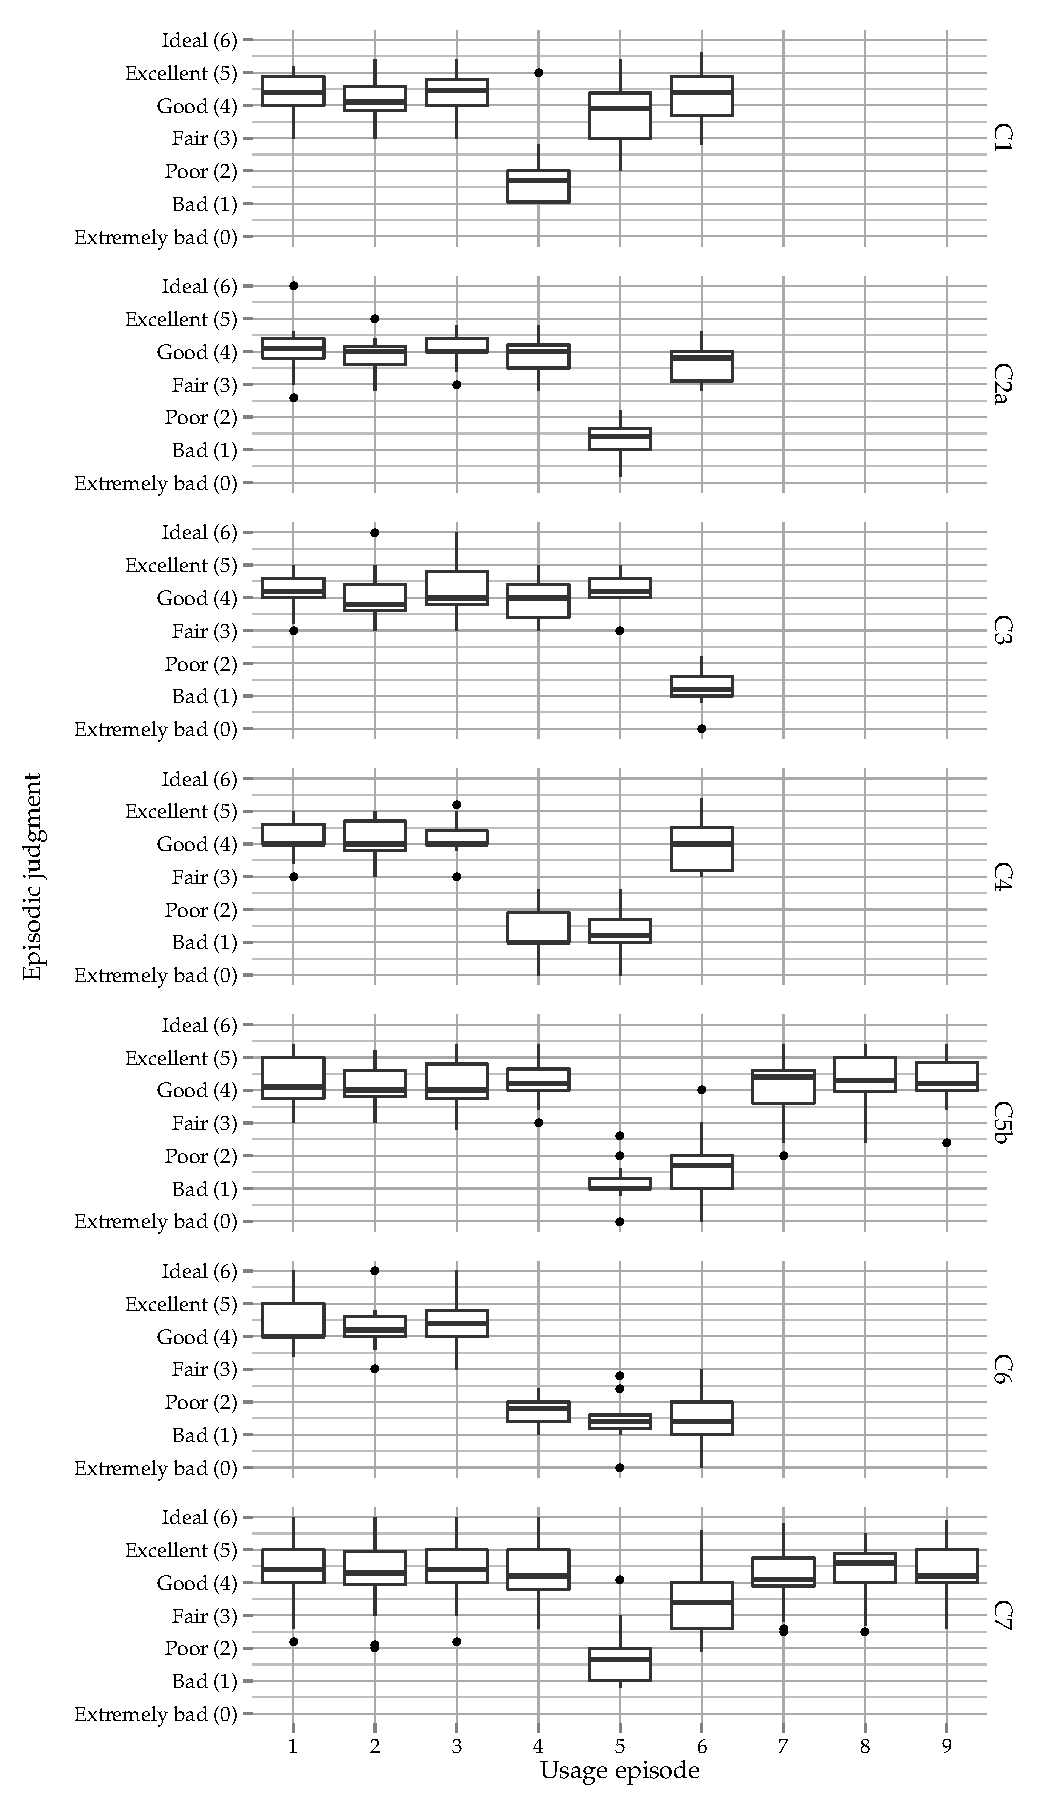
\includegraphics[width=\maxwidth]{figure/plotE1-1} 

\end{knitrout}
	\caption[One session (\E1{}): box plot of the episodic judgments]{One session (\E1{}): box plot of the episodic judgments.}
\end{figure}

\begin{figure}[H]
	\centering
\begin{knitrout}
\definecolor{shadecolor}{rgb}{0.969, 0.969, 0.969}\color{fgcolor}
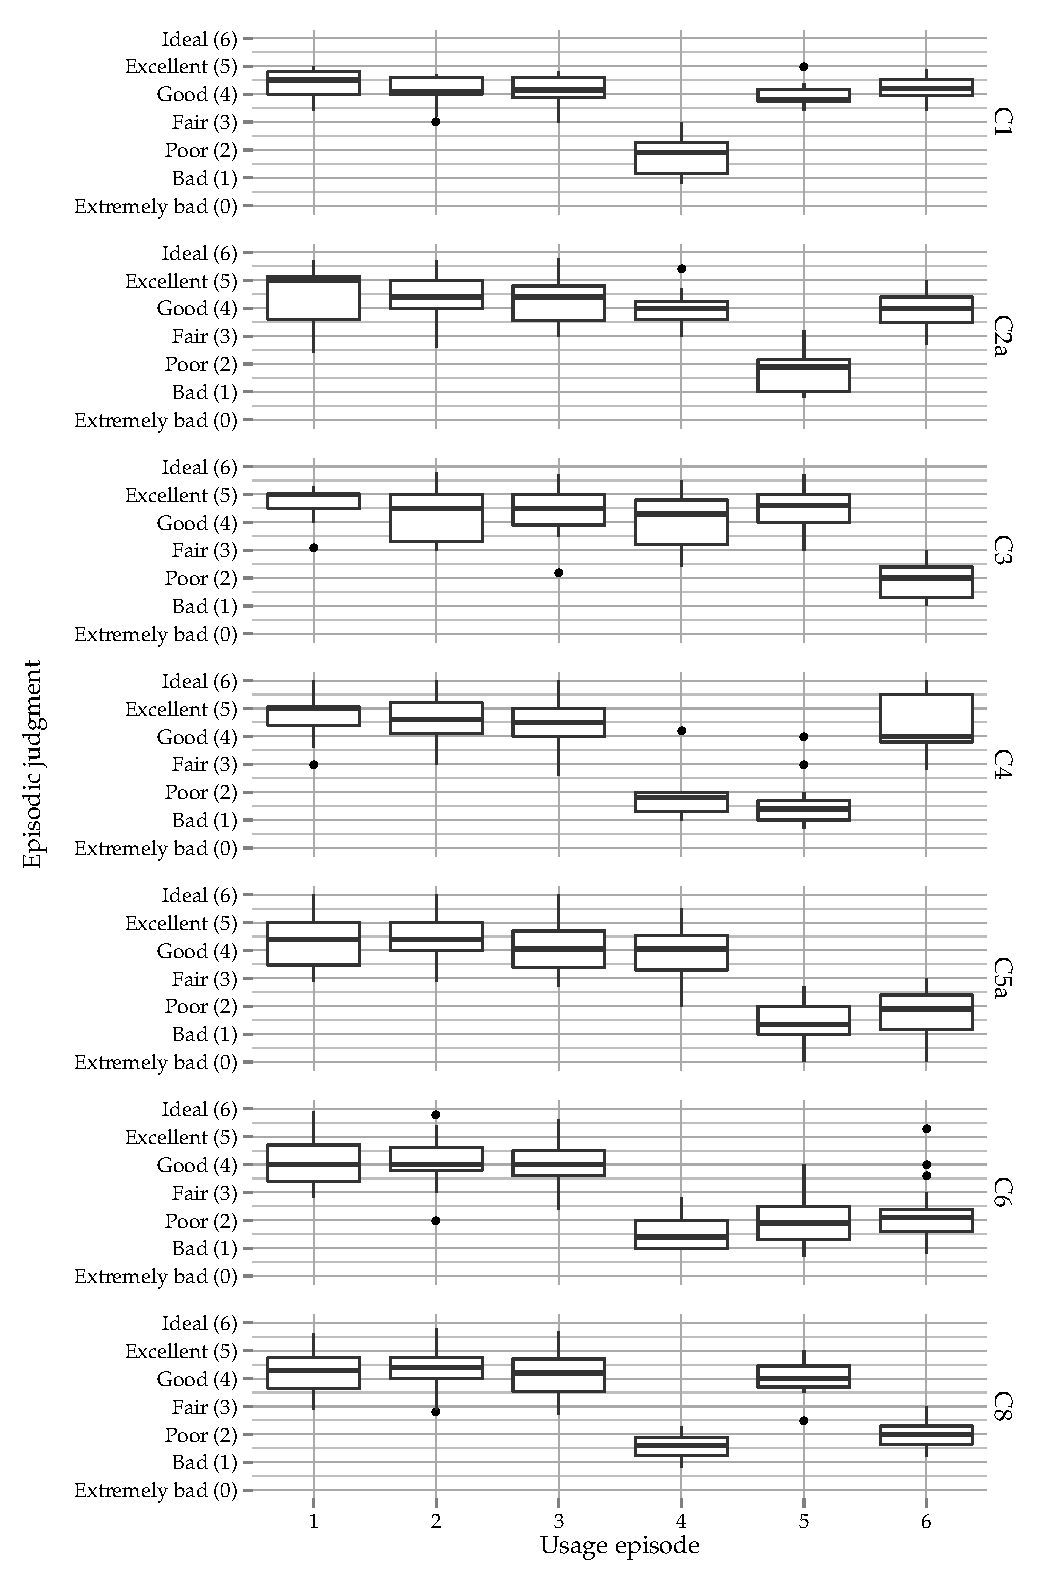
\includegraphics[width=\maxwidth]{figure/plotE2a-1} 

\end{knitrout}
	\caption[One session (\EIIa{}): box plot of the episodic judgments]{One session (\EIIa{}): box plot of the episodic judgments.}	
\end{figure}

\begin{figure}[H]
	\centering
\begin{knitrout}
\definecolor{shadecolor}{rgb}{0.969, 0.969, 0.969}\color{fgcolor}
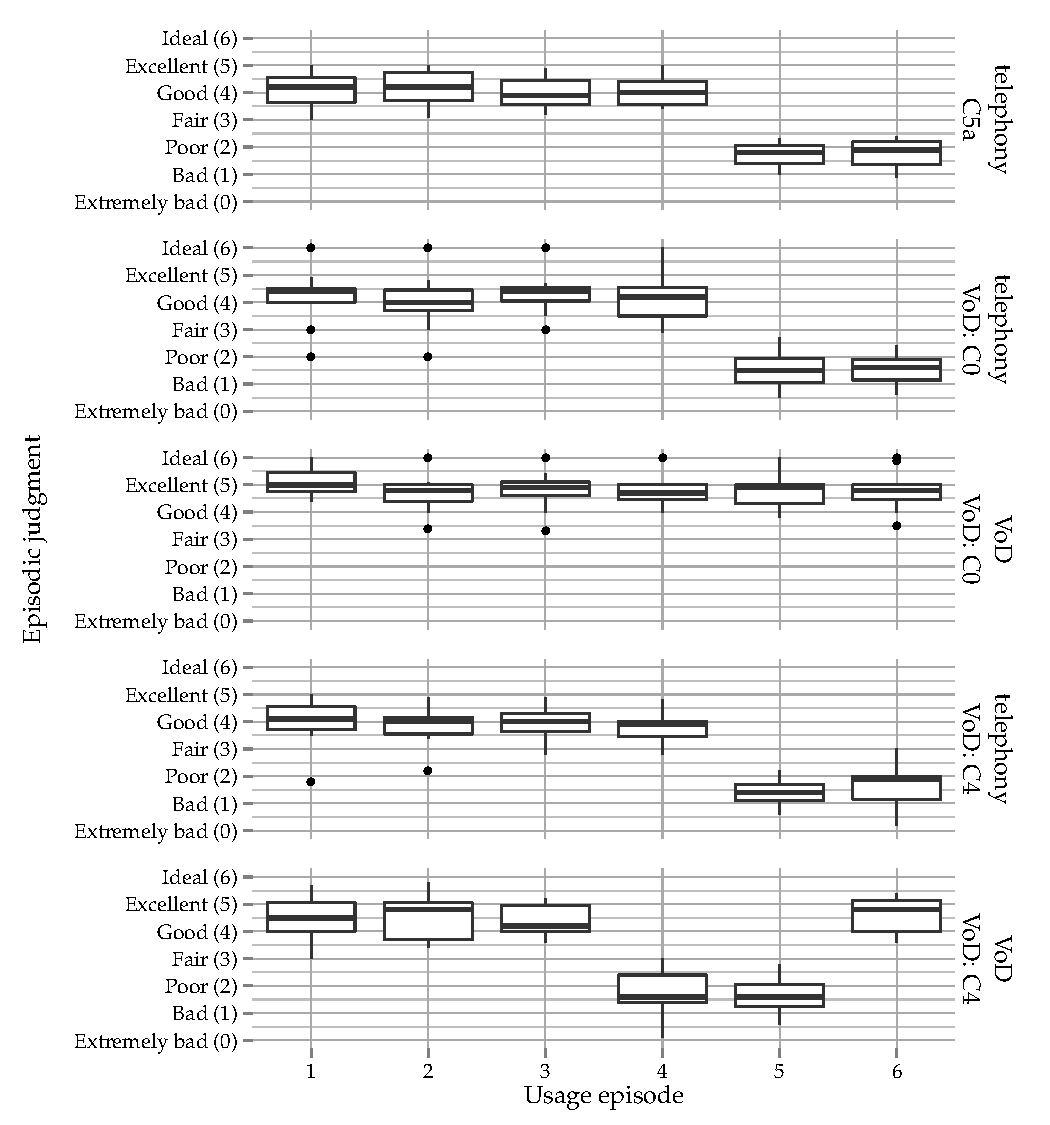
\includegraphics[width=\maxwidth]{figure/plotE2b-1} 

\end{knitrout}
	\caption[One session (\EIIb{}): box plot of the episodic judgments]{One session (\EIIb{}): box plot of the episodic judgments.}
\end{figure}

\begin{figure}[H]
	\centering
\begin{knitrout}
\definecolor{shadecolor}{rgb}{0.969, 0.969, 0.969}\color{fgcolor}
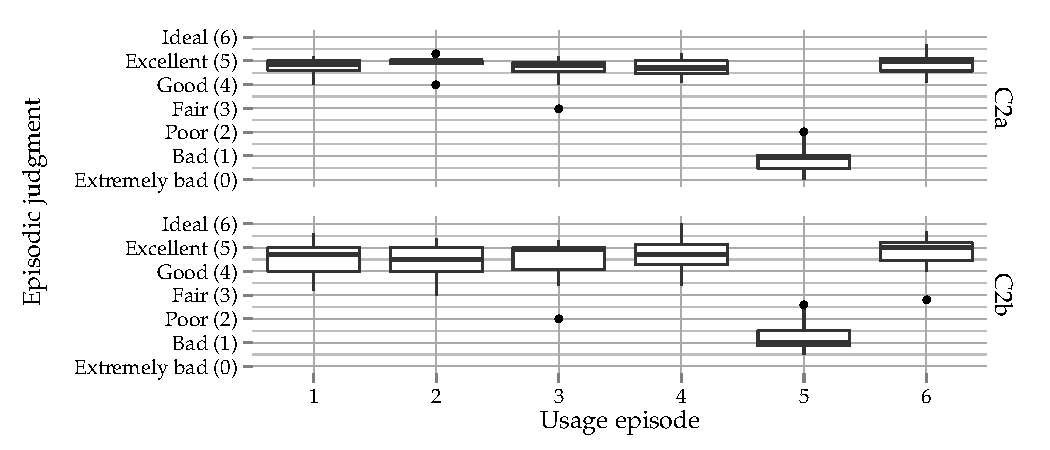
\includegraphics[width=\maxwidth]{figure/plotE3-1} 

\end{knitrout}
	\caption[One session (\E3{}): box plot of the episodic judgments]{One session (\E3{}): box plot of the episodic judgments.}
\end{figure}

\begin{figure}[H]
	\centering
\begin{knitrout}
\definecolor{shadecolor}{rgb}{0.969, 0.969, 0.969}\color{fgcolor}
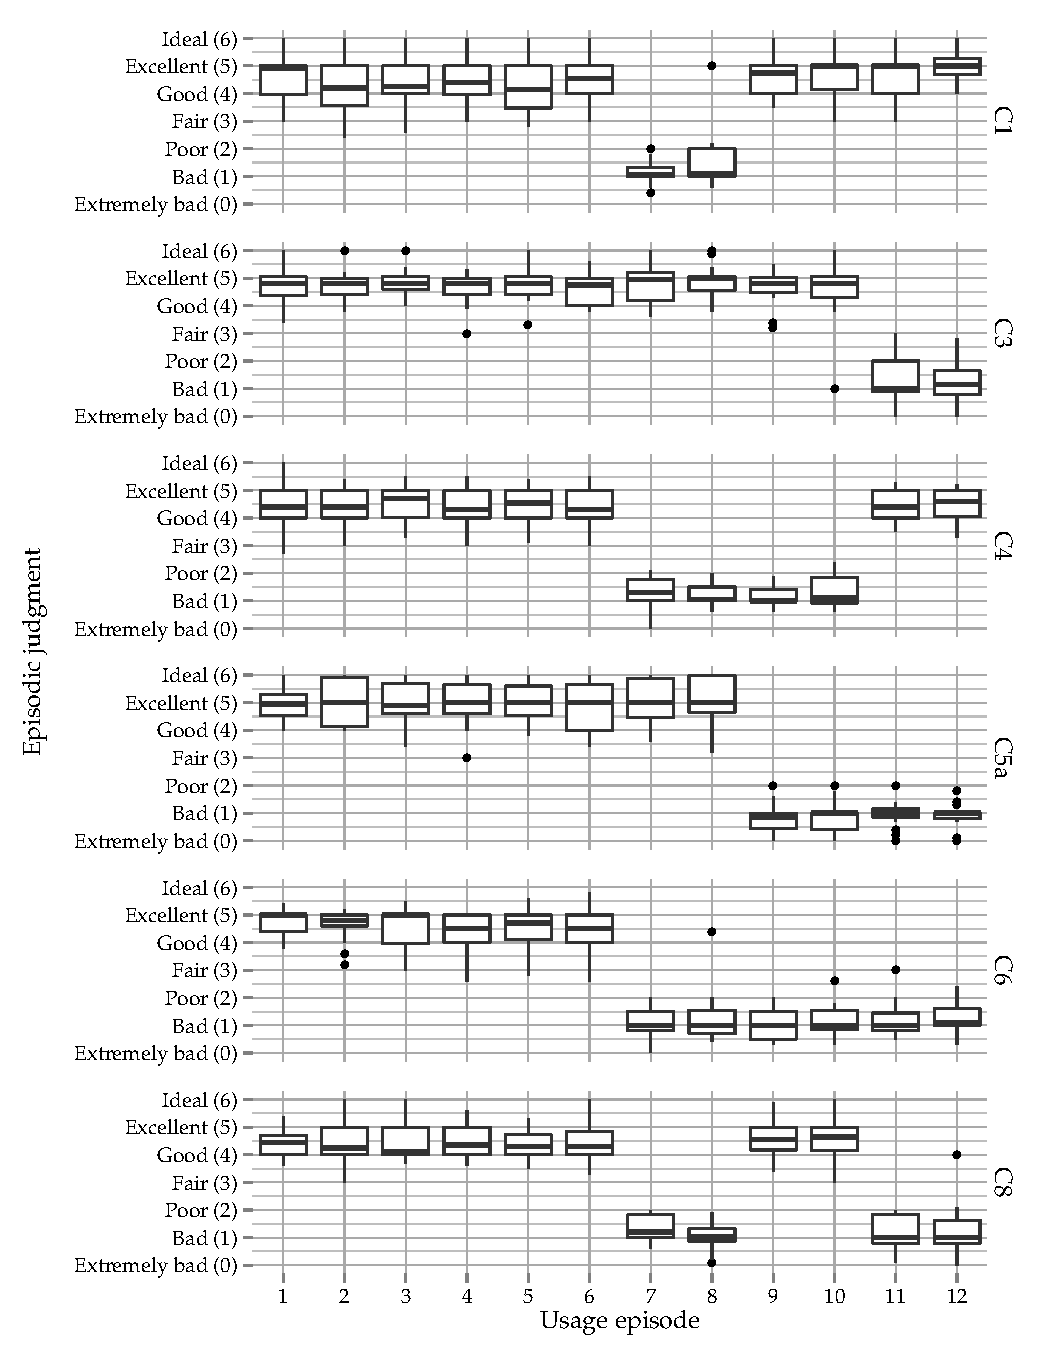
\includegraphics[width=\maxwidth]{figure/plotE6-1} 

\end{knitrout}
	\caption[Multiple days (\E6{}): box plot of episodic judgments]{Multiple days (\E6{}): box plot of episodic judgments.}
\end{figure}

\section{Multi-episodic Judgments}

\begin{table}[H]
	\centering
	\caption[Multi-episodic judgments per condition and experiment for \E1{}, \EIIa{}, \EIIb{}, and \E3{}]{Multi-episodic judgments per condition and experiment for \E1{}, \EIIa{}, \EIIb{}, and \E3{}.}
	\begin{tabulary}{\textwidth}{C|C|C|C|C}
	Experiment &  Condition & \multicolumn{3}{c}{Multi-episodic judgment} \\
	& & 3rd episode & 6th episode & 9th episode \\
	\midrule
	\E1{} & \C1{} 	& 4.4 (0.6) 		& 3.7 (0.6) 		& -  \\
	\hline
	\E1{} & \CIIa{} & 4.1 (0.4) 	& 3.2 (0.6) 	& - \\
	\hline
	\E1{} & \C3{} 	& 4.3 (0.8) 		& 3.1 (0.8) 		& -  \\
	\hline
	\E1{} & \C4{} 	& 4.2 (0.5) 		& 2.9 (0.5) 		& - \\ 
	\hline
	\E1{} & \CVb{} 	& 4.1 (0.6) 	& 2.3 (0.9) 	& 3.6 (0.6)\\
	\hline	
	\E1{} & \C6{} 	& 4.3 (0.7) 		& 2.1 (0.7) 		& - \\
	\hline
	\E1{} & \C7{} 	& 4.4 (0.8) 		& 3.1 (0.7) 		& 4.1 (0.6)\\
	\hline
	\hline
	\EIIa{} & \C1{} 	& 4.3 (0.6) 		& 3.6 (0.5) 		& - \\
	\hline
	\EIIa{} & \CIIa{} & 4.4 (0.7) 	& 3.5 (0.5) 	& - \\
	\hline
	\EIIa{} & \C3{} 	& 4.3 (0.8) 		& 3.5 (0.5) 		& - \\
	\hline
	\EIIa{} & \C4{} 	& 4.8 (0.7) 		& 3.0 (0.9) 		& - \\
	\hline
	\EIIa{} & \CVa{} 	& 4.2 (0.8) 	& 2.4 (0.9) 	&  - \\
	\hline	
	\EIIa{} & \C6{} 	& 4.1 (0.8) 		& 2.5 (0.8) 		& - \\
	\hline
	\EIIa{} & \C8{} 	& 4.3 (0.8) 		& 2.5 (0.6) 		& - \\
	\hline
	\hline
	\EIIb{} (telephony) 	& telephony: \CVa{}; \ac{VoD}: - & 4.2 (0.5) & 2.6 (0.8) 		& - \\
	\hline
	\EIIb{} (telephony) 	& telephony: \CVa{}; \ac{VoD}: \C0{} & 3.8 (1.3) & 2.7 (0.7) 	& - \\
	\hline
	\EIIb{} (\ac{VoD})		& telephony: \CVa{}; \ac{VoD}: \C0{} 	& 4.4 (0.8) 		& 4.7 (0.6) 		& - \\
	\hline
	\EIIb{} (telephony) 	& telephony: \CVa{}; \ac{VoD}: \C4{} & 4.0 (0.7) 	& 2.7 (0.8) 	& - \\
	\hline
	\EIIb{} (\ac{VoD}) 	& telephony: \CVa{}; \ac{VoD}: \C0{}	& 4.4 (0.9) 		& 3.5 (0.8) 		& - \\
	\hline
	\hline	
	\E3{} & \CIIa{} 	& 4.8 (0.3) 		& 3.9 (0.6)	& - \\
	\hline
	\E3{} & \CIIb{} & 4.5 (0.8) 	& 3.7 (0.6) 	& - \\
	\end{tabulary}
	\label{appendix:lab:multiepisodicResult}
\end{table}



%\chapter{Content}
%\section{\acs{SCS} used in \E1, \E2a, \E2b, and E3}
%\begin{table}[h]
%	\centering
%	\caption{The \acs{SCS} used in \E1, \E2, and \E3 were taken from \citet{itu-t_recommendation_p.805_subjective_2007} and outdated information updated. The scenario of episode 4 was changed from a flight information and booking task to a change of booking task.}
%	\begin{tabular}{c|c|c}
%	Episode & Title & Page \\
%	\hline
%	1 & Travel Agent (German: Reisebüro) & p.\,16f \\
%	2 & Rail Travel Information (German: Bahnauskunft) & p.\,18f \\
%	3 & Theater Box office (German: Theaterkasse) & p.\,30f \\
%	4 & Renting a car (German: Autovermietung) & p.\,26f \\
%	5 & Information on Flights (German: Flugumbuchung) & Based on p.\,24f \\
%	6 & Eye Specialist's Appointment (German: Arzttermin) & p.\,50f \\
%	7 & Pizza Service (German: Pizzaservice) & p.\,38f \\
%	8 & Flat to Let (German: Wohnungsanzeige) & p.\,46f \\
%	9 & Booking an Apartment (German: Appartmentreservierung) & p.\,36f \\
%	\end{tabular}
%	\label{tab:appendix:labsct}
%\end{table}
